\section{Dise\~no}

\subsection{Descripci\'on informal}

El sistema desarrollado consiste en dos programas que pueden ser invocados mediante línea de comandos, \textsf{generar-base.py} y \textsf{simular-partido.py}. El primero tiene la finalidad de generar una base de datos donde se persisten tanto las estadísticas de los jugadores como los libros de jugadas de los directores técnicos, y el segundo ejecuta una simulación en base a un archivo de entrada de tipo JSON conteniendo la composición de los equipos a enfrentarse.

El programa \textsf{generar-base.py} genera un archivo de extension \texttt{db} utilizando el motor SQLite, y luego popula la base datos con estadísticas de un conjunto de jugadores desde la API oficial de la NBA\footnote{API oficial de la NBA: http://stats.nba.com}. Adicionalmente, se definen cuáles jugadas tiene cada director técnico en su libro de jugadas, con su correspondiente nivel de preferencia (un número en una escala arbitraria entre 1 y 5).

Una vez generada la base de datos, ya se puede utilizar el programa \textsf{simular-partido.py} para realizar una simulación. El mismo lee la conformación de los equipos, y ejecuta la simulación imprimiendo por salida estándar el log generado durante la misma.

\subsection{Modelo de la simulación}

El simulador está implementado en el módulo Python \textsf{simulacion}, el cual consiste de una serie de clases de tipo Simulador, representando cada una ĺa simulación de un partido de básquet a distintos niveles de detalle. Hay un total de cuatro niveles de simulación:

\begin{enumerate}
  \item \textsf{SimuladorPartido} representa la simulación de un partido en su totalidad; una ronda de 40 turnos, seguida por tantas rondas de 6 turnos como sean necesarias hasta que el partido tenga un ganador.
  \item \textsf{SimuladorTurno} representa la simulación de un turno dentro de un partido, estando compuesto por una sucesión de jugadas.
  \item \textsf{SimuladorJugada} representa la simulación de una jugada dentro de un turno, estando compuesta por una sucesión de momentos.
  \item \textsf{SimuladorMomento} representa la simulación de un instante dentro de una jugada, en el cual el jugador atacante en posesión de la pelota realiza una acción, y un jugador defensor realiza la acción defensiva correspondiente.
\end{enumerate}

Todos los niveles son polimórficos con respecto al método \texttt{simular}. La implementación de éste método sigue el mismo esquema en todos los niveles, y es el siguiete:

\begin{enumerate}
  \item Registrar comienzo de la simulación de este nivel.
  \item Simular una o más ejecuciones del nivel inmediatamente inferior.
  \begin{enumerate}
  \item[2.1.] Por cada ejecución del nivel inmediatamente inferior, actualizar el estado de este nivel.
  \end{enumerate}
  \item Registrar fin de la simulación de este nivel.
\end{enumerate}

\subsection{Diagramas de objeto}

Incluimos un diagrama de objetos por cada nivel de simulación, representando el estado que se mantiene en cada uno de ellos, así como su interacción con el nivel inmediatamente inferior (si aplica).

En cada diagrama, se indican en rojo las relaciones de conocimiento que surgen del pasaje de parámetros en la construcción. Así podemos ver el estado con el que se construye cada uno de los niveles de simulación.

\subsubsection{Simulador de Partido}
Diagrama de objetos de un simulador de partido, para el caso en que un turno termina en conversi\'on triple, justo antes que el resultado del turno actualice el simulador de partido.

\begin{center}
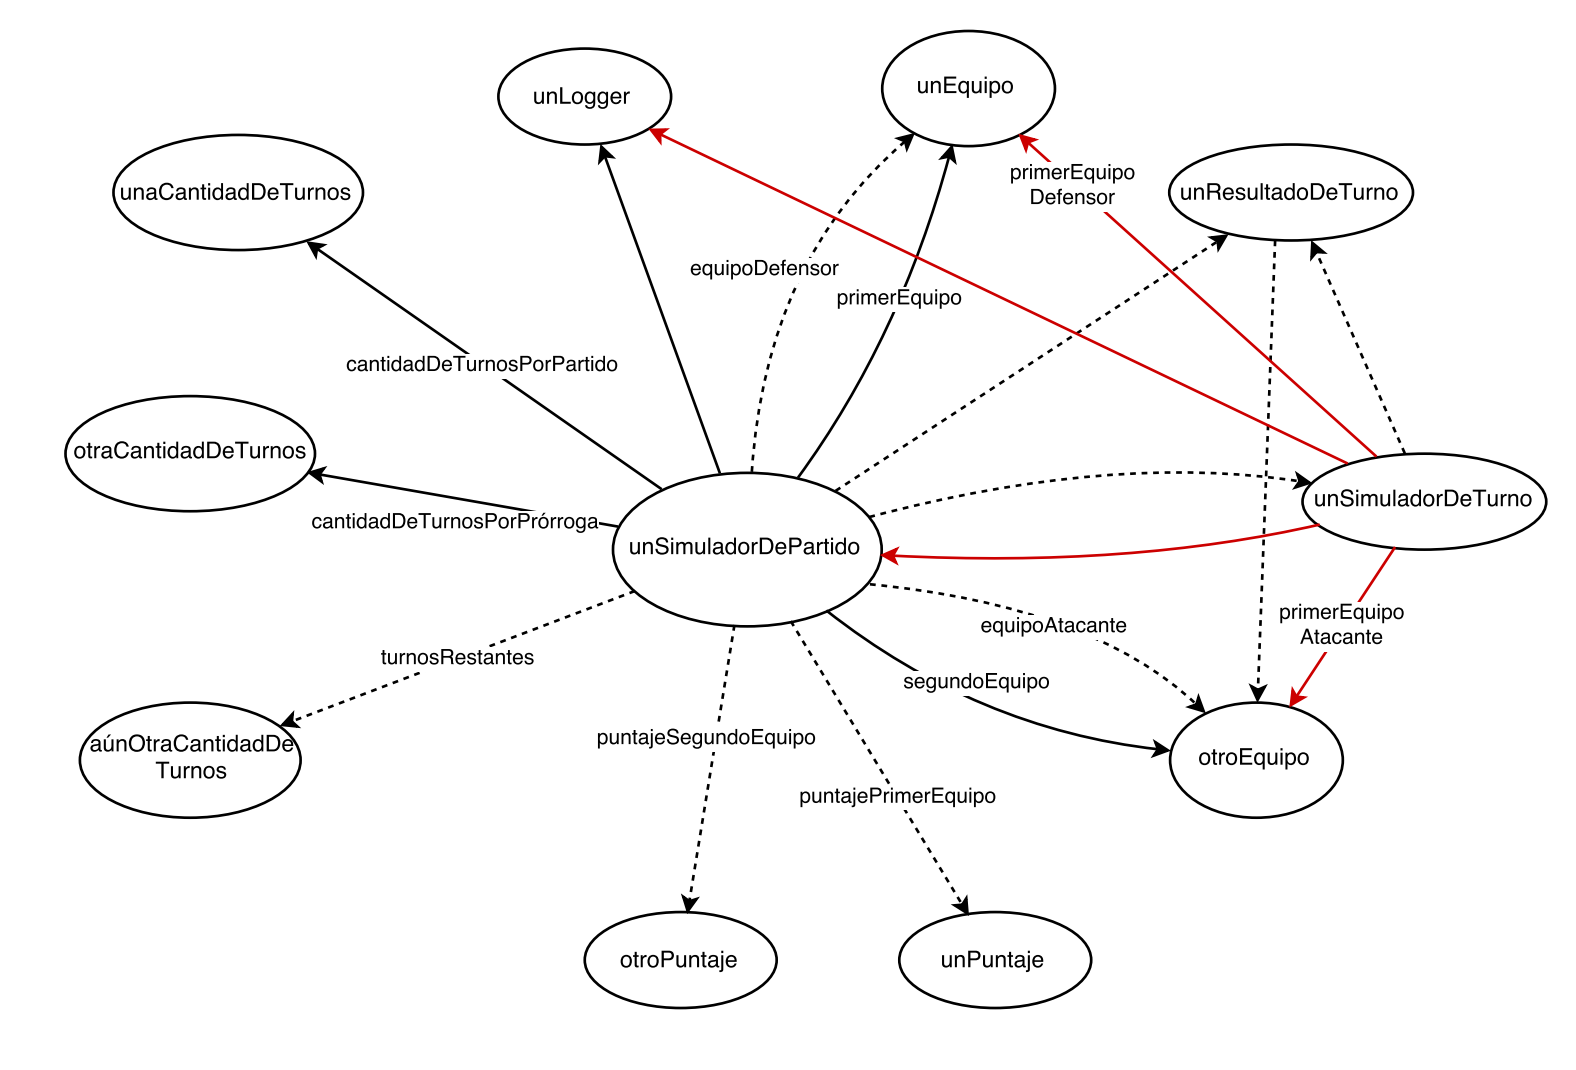
\includegraphics[width=15cm]{diagramas/DO1}
\end{center}

Diagrama de objetos luego de actualizar el simulador de partido.

\begin{center}
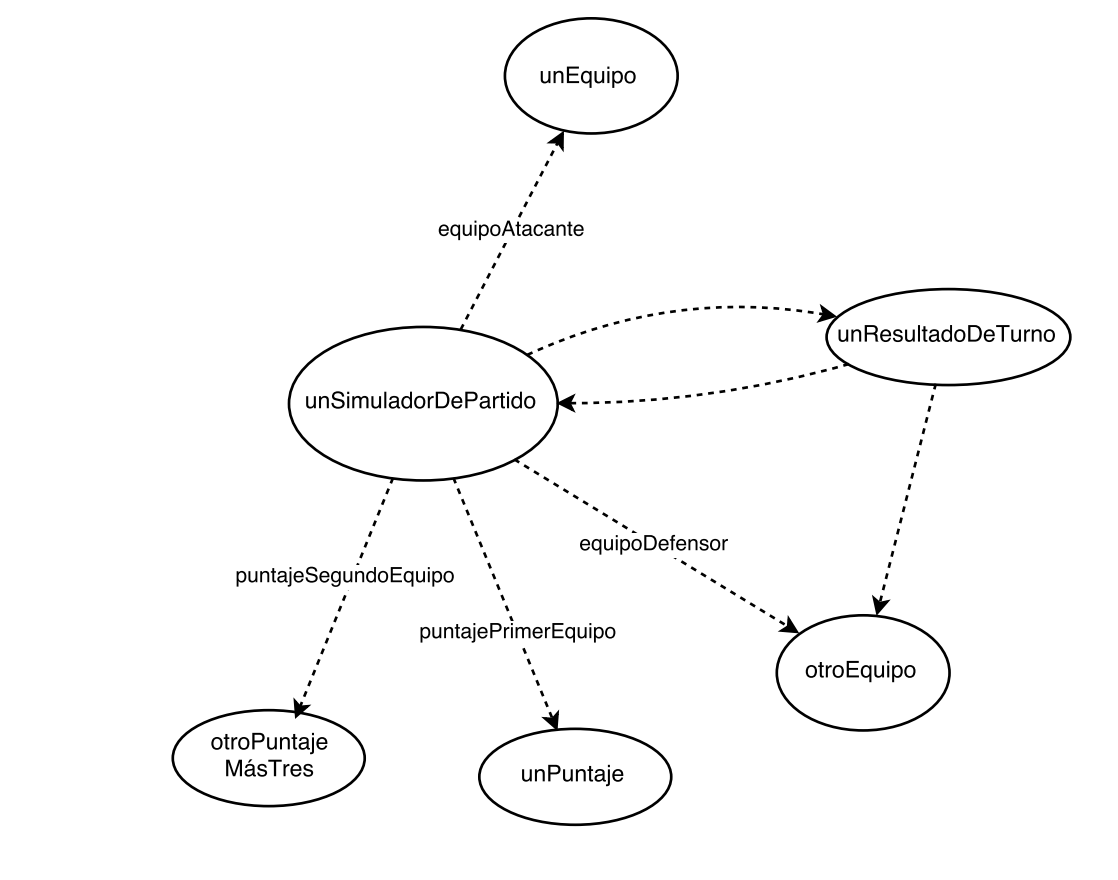
\includegraphics[width=15cm]{diagramas/DO2}
\end{center}

\subsubsection{Simulador de Turno}

Diagrama de objetos de un simulador de turnos, para el caso en que una jugada termina en pase robado, justo antes que el resultado de la jugada actualice el simulador de turno.

\begin{center}
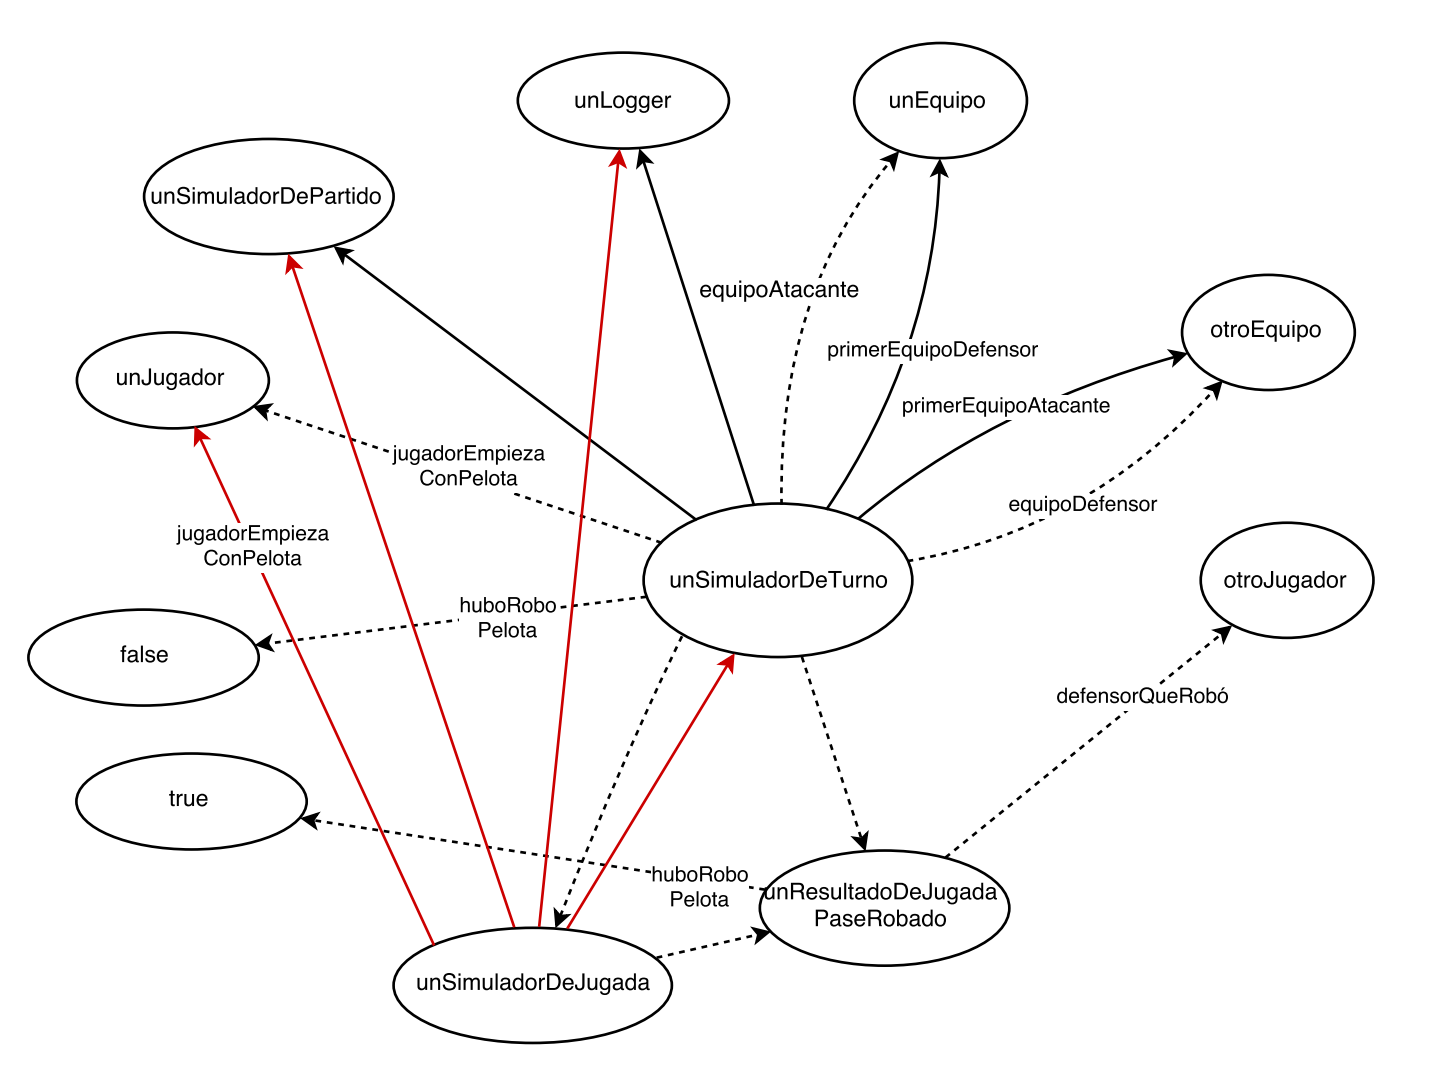
\includegraphics[width=15cm]{diagramas/DO3}
\end{center}

Diagrama de objetos luego de actualizar el turno.

\begin{center}
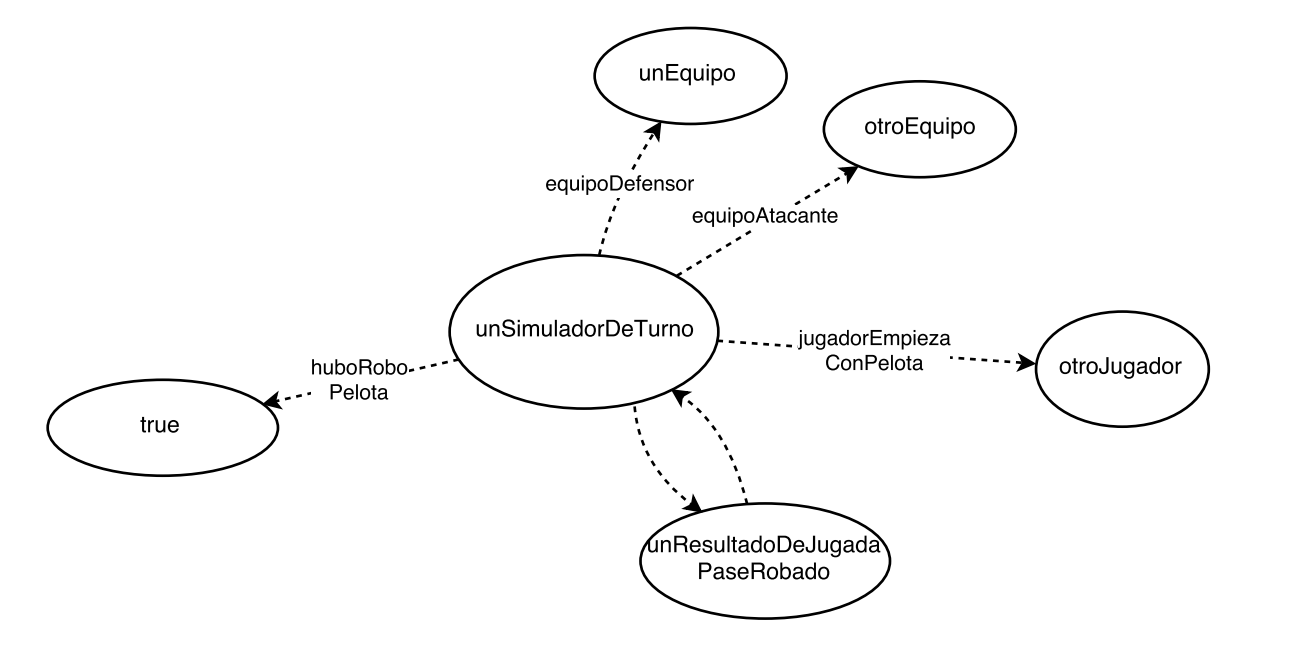
\includegraphics[width=15cm]{diagramas/DO4}
\end{center}

Diagrama de objetos luego de la \'ultima jugada del turno.

\begin{center}
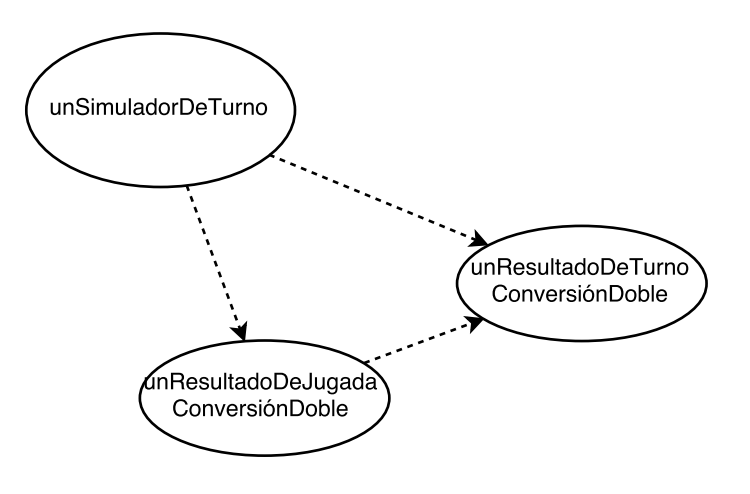
\includegraphics[width=8cm]{diagramas/DO5}
\end{center}

\subsubsection{Simulador de Jugada}

Diagrama de objetos de un simulador de jugada, para el caso en que un momento termina en pase exitoso, justo antes que el resultado del momento
actualice el simulador de jugada.

\begin{center}
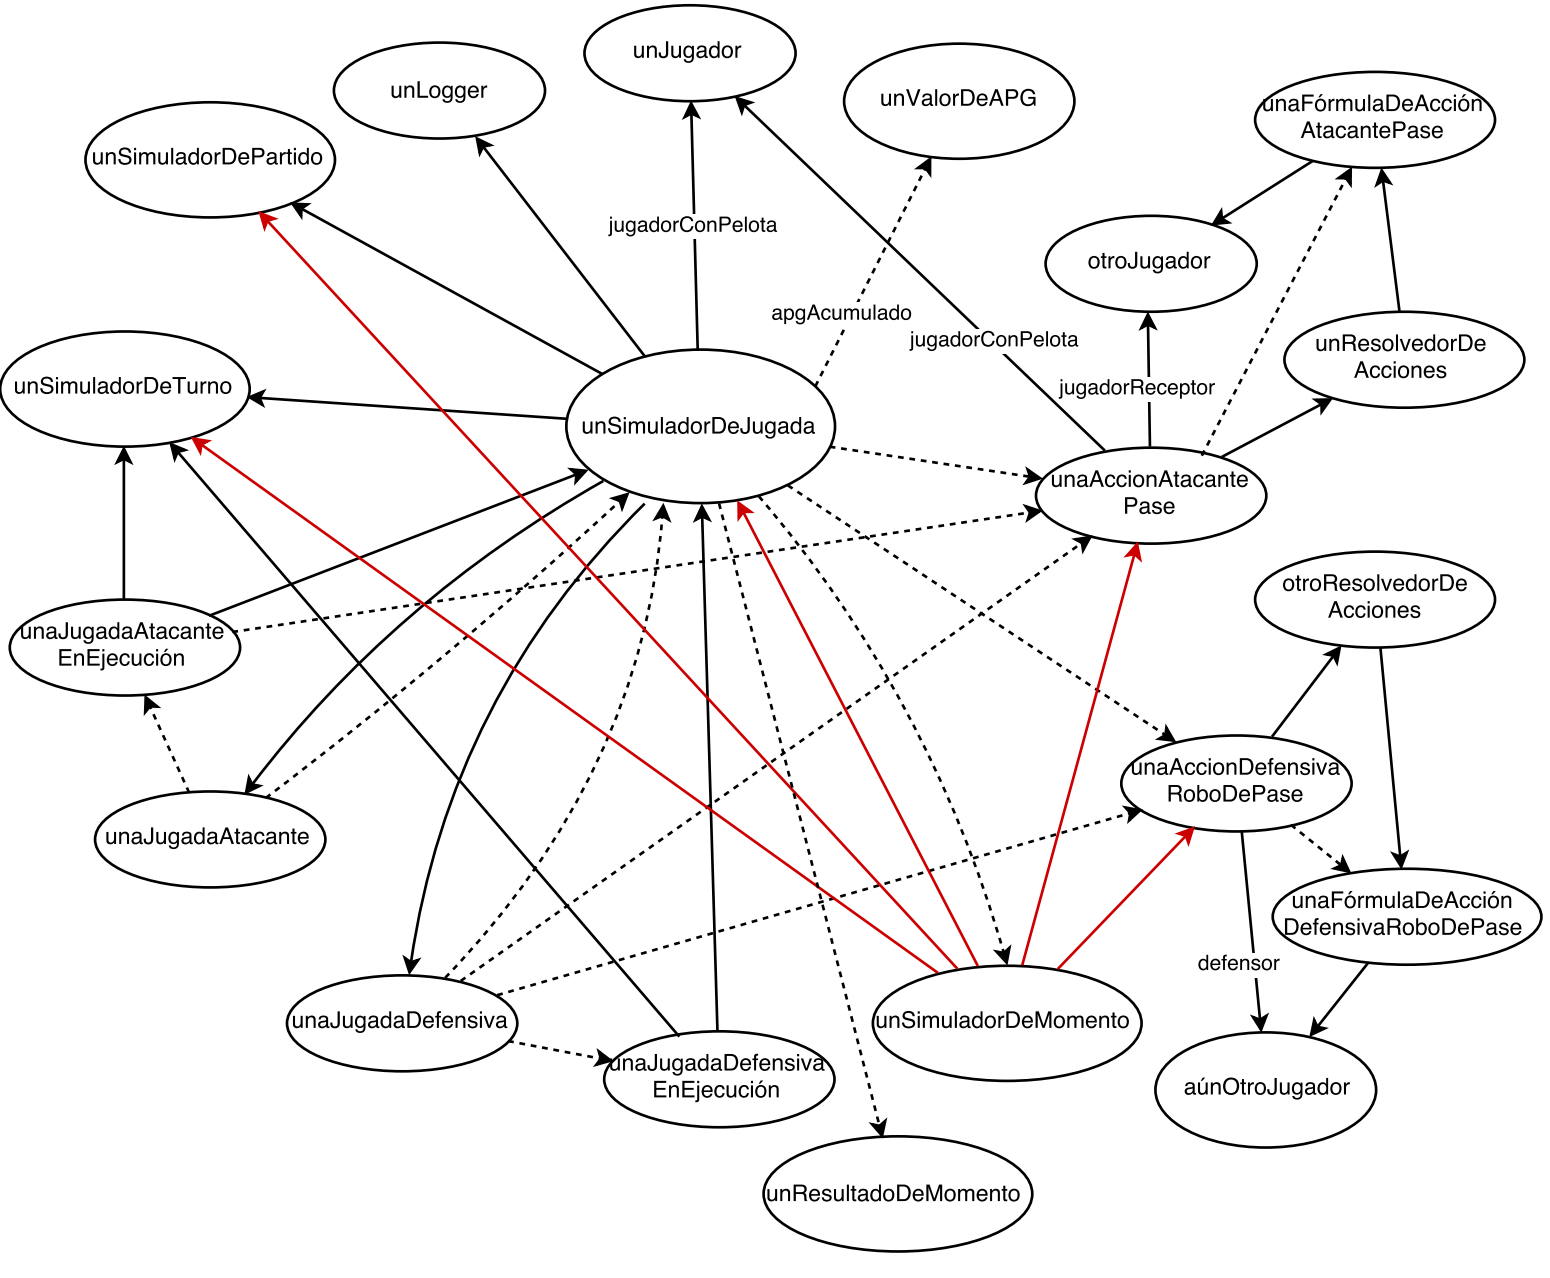
\includegraphics[width=15cm]{diagramas/DO6}
\end{center}

Diagrama de objetos luego de actualizar el simulador de jugada.

\begin{center}
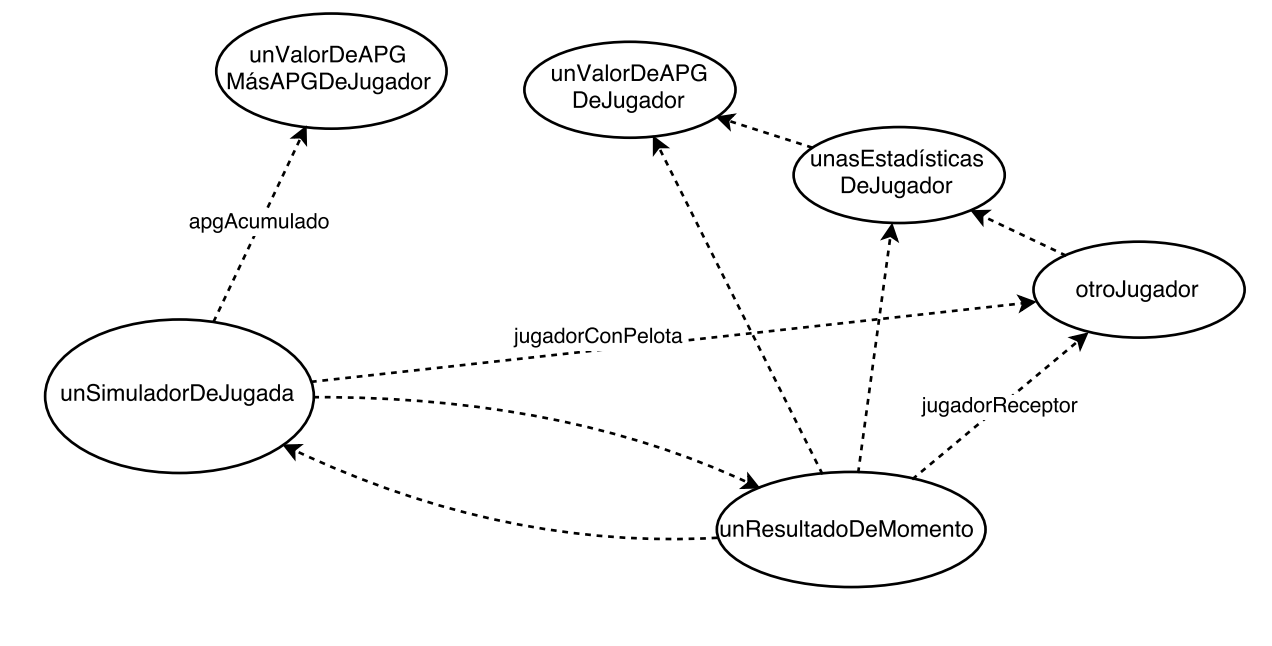
\includegraphics[width=15cm]{diagramas/DO7}
\end{center}

\subsubsection{Simulador de Momento}

Diagrama de objetos de un simulador de momento, para el caso de un pase fallido por robo de pelota.

\begin{center}
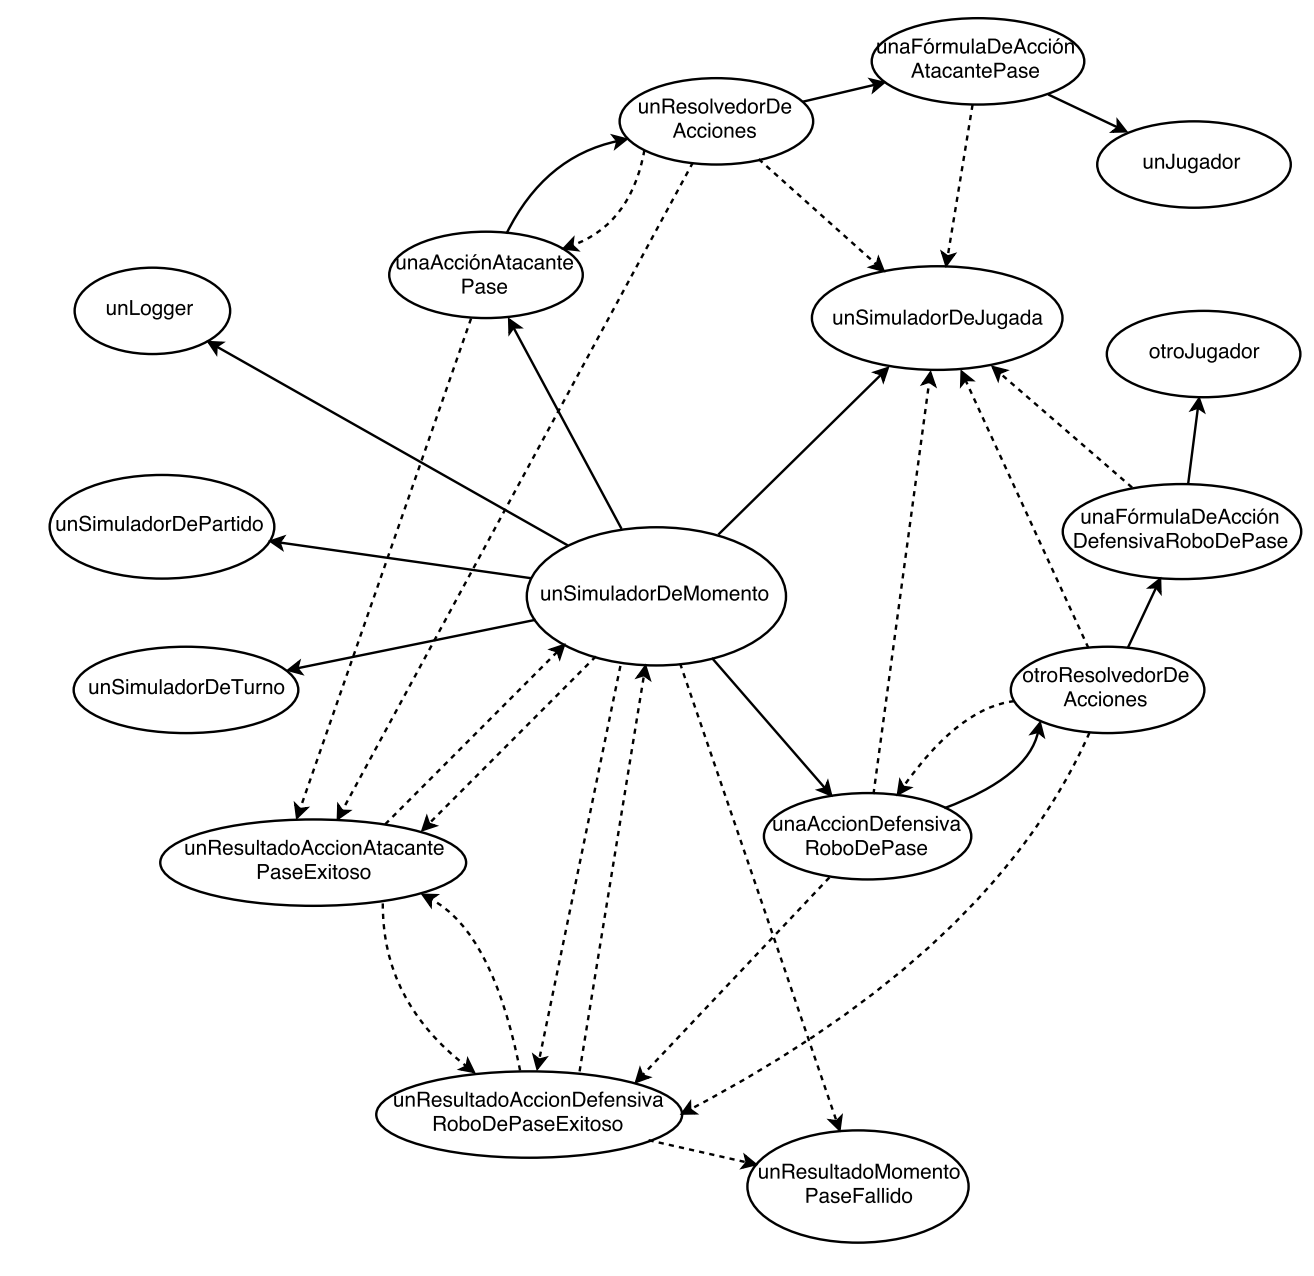
\includegraphics[width=15cm]{diagramas/DO8}
\end{center}

\subsection{Diagrama de secuencia}
% presentación de la razón de ser
Incluimos un diagrama de secuencia que abarca la secuencia de colaboraciones que desencadena el envío
del mensaje jugar (simular, finalmente) a la clase SimuladorMomento con el objetivo de mostrar claramente
la interacción mediante la cual se resuelven las acciones atacantes y defensivas en un Momento particular.

% explicación del diagrama
El diagrama muestra que para simular un MomentoDeJugada se deben obtener el resultado de simular ambas acciones
utilizando las fórmulas de resolución de acciones, ofensiva y defensiva, independientemente. Una vez definido el resultado de
cada una de las acciones mediante un double dispatch se obtiene el resultado del momento. El double dispatch se realiza entre
el resultado de la acción atacante al cual se le envia el mensaje obtenerResultadoMomento recibiendo como colaborador externo
al resultado de la acción defensiva. El resultado de la acción atacante invoca el mensaje correspondiente sobre el resultado de
la acción defensiva en función de su propio tipo. Finalmente, el resultado de acción defensiva devolverá el resultado del momento
en función de su propio tipo, completando el double dispatch.

\begin{center}
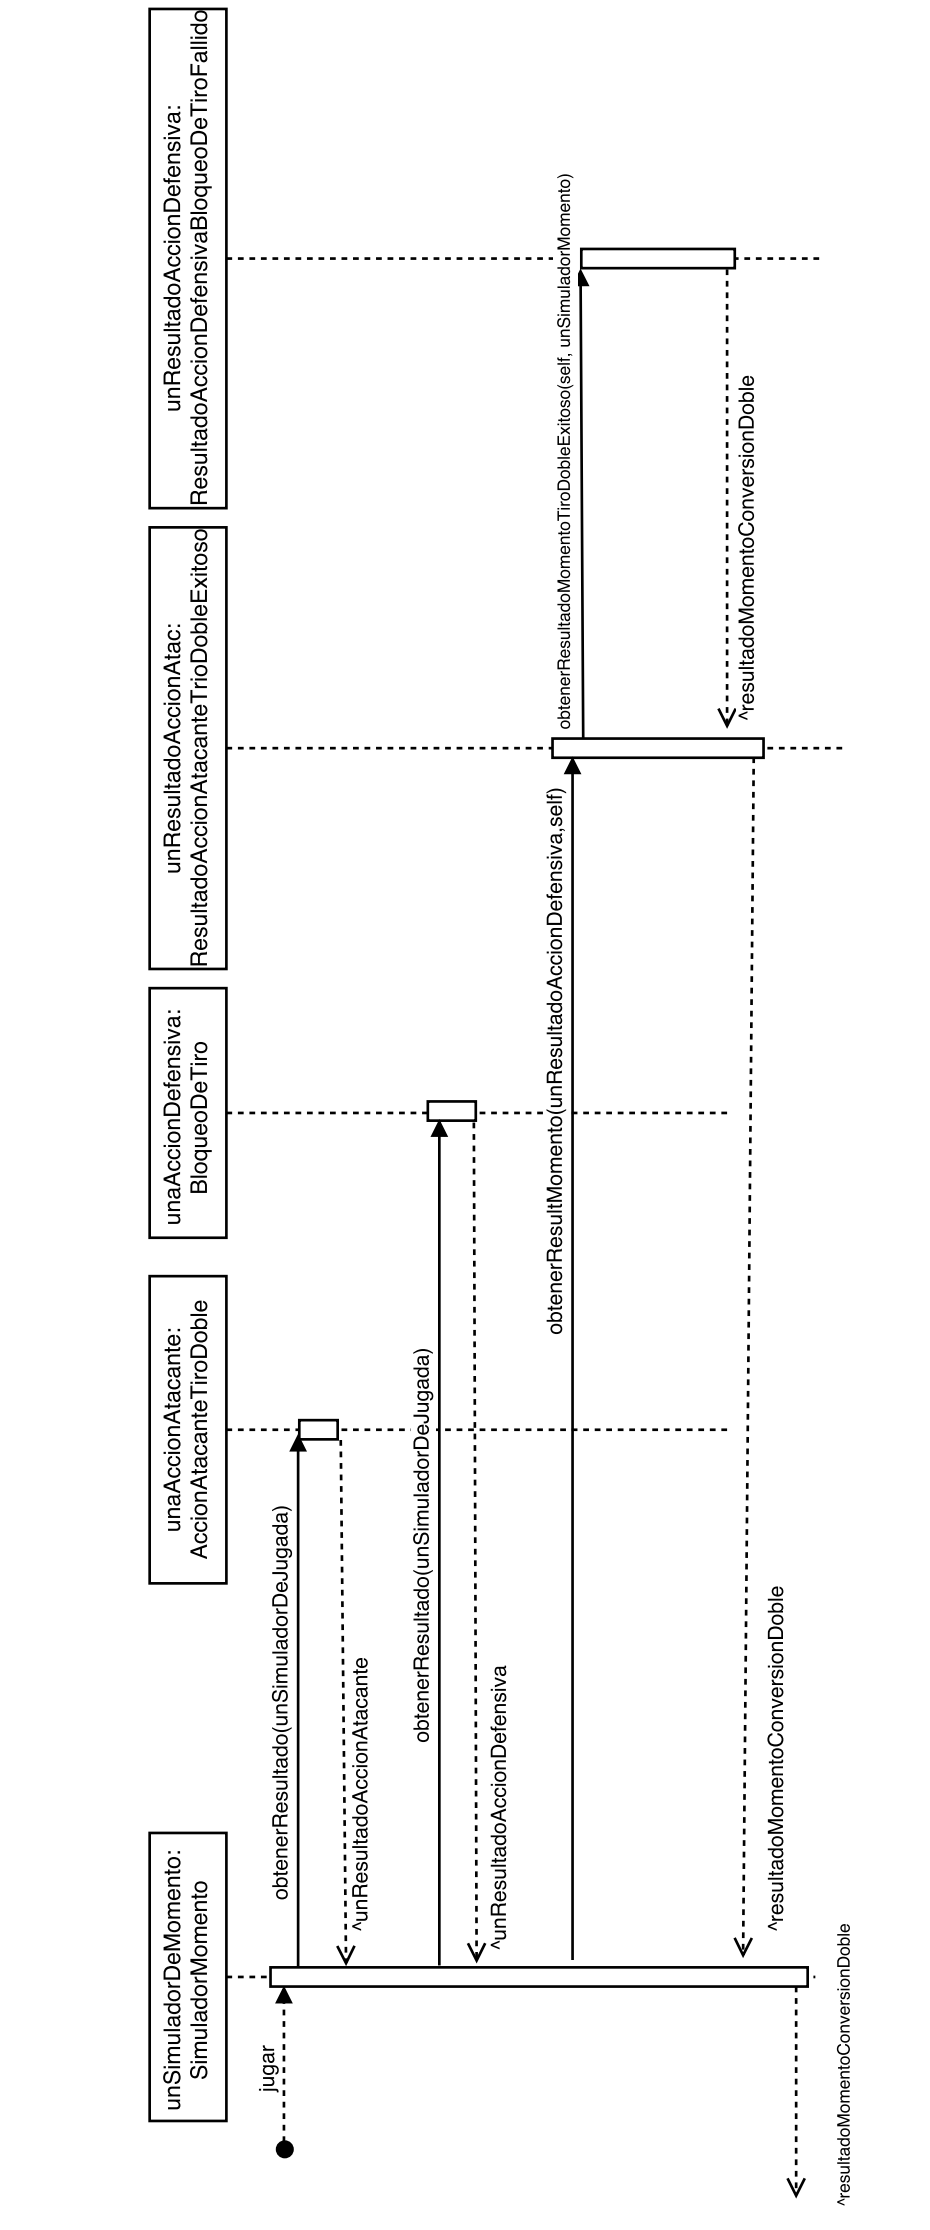
\includegraphics[width=8cm]{diagramas/secuencia}
\end{center}

\newpage

\subsection{Diagramas de clase}

El correspondiente diagrama de clases lo enviamos adjunto con el informe a causa del tamaño del gr\'afico. A continuación, realizamos un par de aclaraciones sobre el g\'afico:

\begin{enumerate}
  \item Agregamos clases en color verde, estas clases son clases replicadas, es decir, clases que duplicamos para hacer mas legible el diagrama.
  \item Los conectores de herencia estan hechos con flechas de tamaño mas grande que las comunes, de esta forma el diagrama es mas legible.
\end{enumerate}
